\goal The goal of this part is to successfully build a new image starting from an isolated kernel. An image is a snapshot of living objects binary saved in a file. They basically contains classes and some living instances.
%\sd{Explain Special Objects array}
%done in the Smalltalk presentation part

\problems
\begin{itemize}
	\item Which technique should we use to create the image ?
	\item How to successfully replace the \gls{Special Objects Array} ?
\end{itemize}

\solutions
\begin{figure}[ht]
	\centering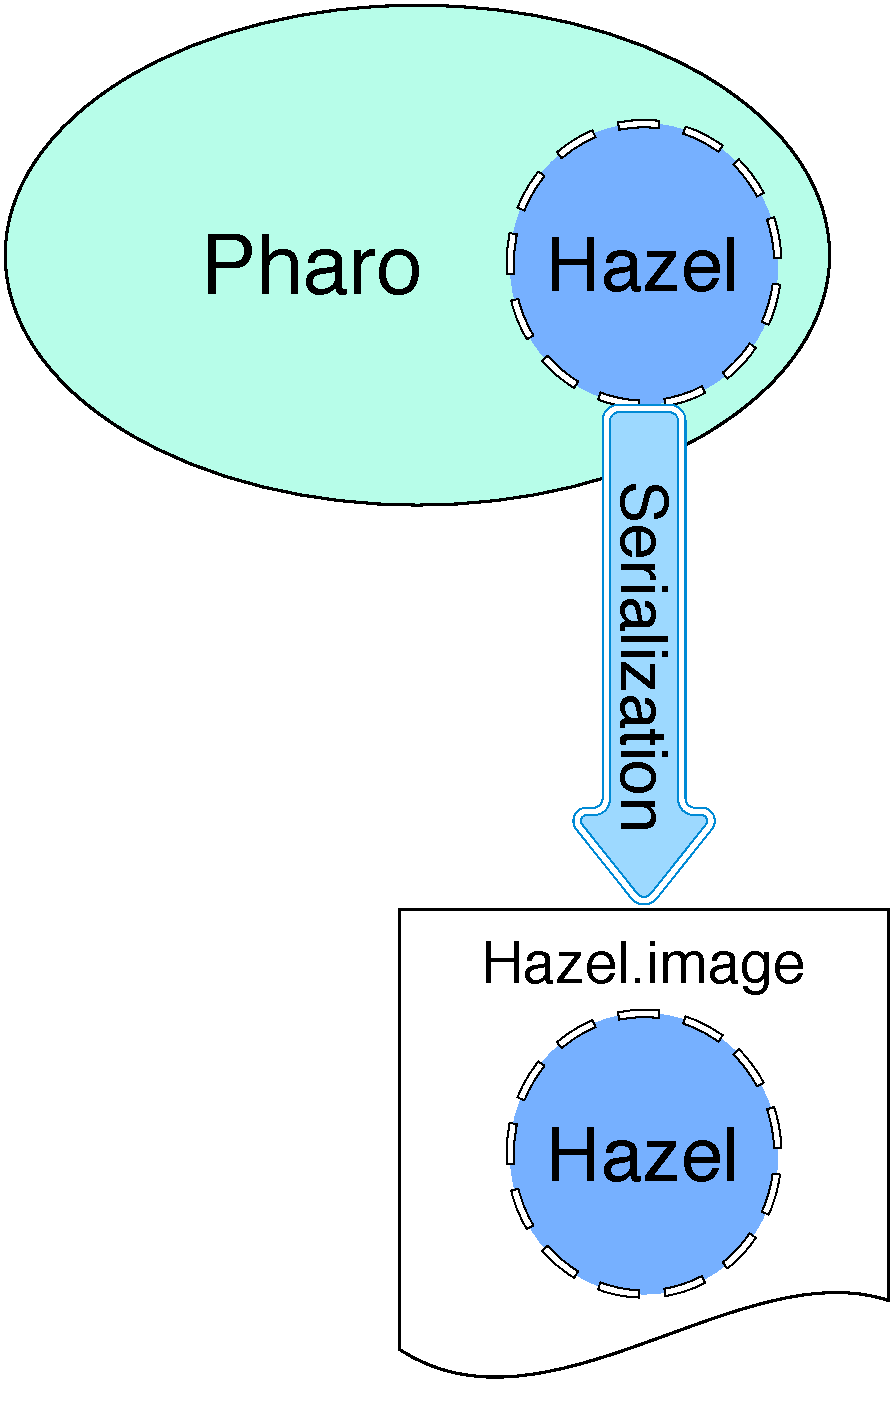
\includegraphics[width = 4.5cm]{figures/MSSolution}
	\caption{Micro Squeak - Serialization of needed objects}
	\label{MSSolution}
\end{figure}
\begin{figure}[ht]
	\centering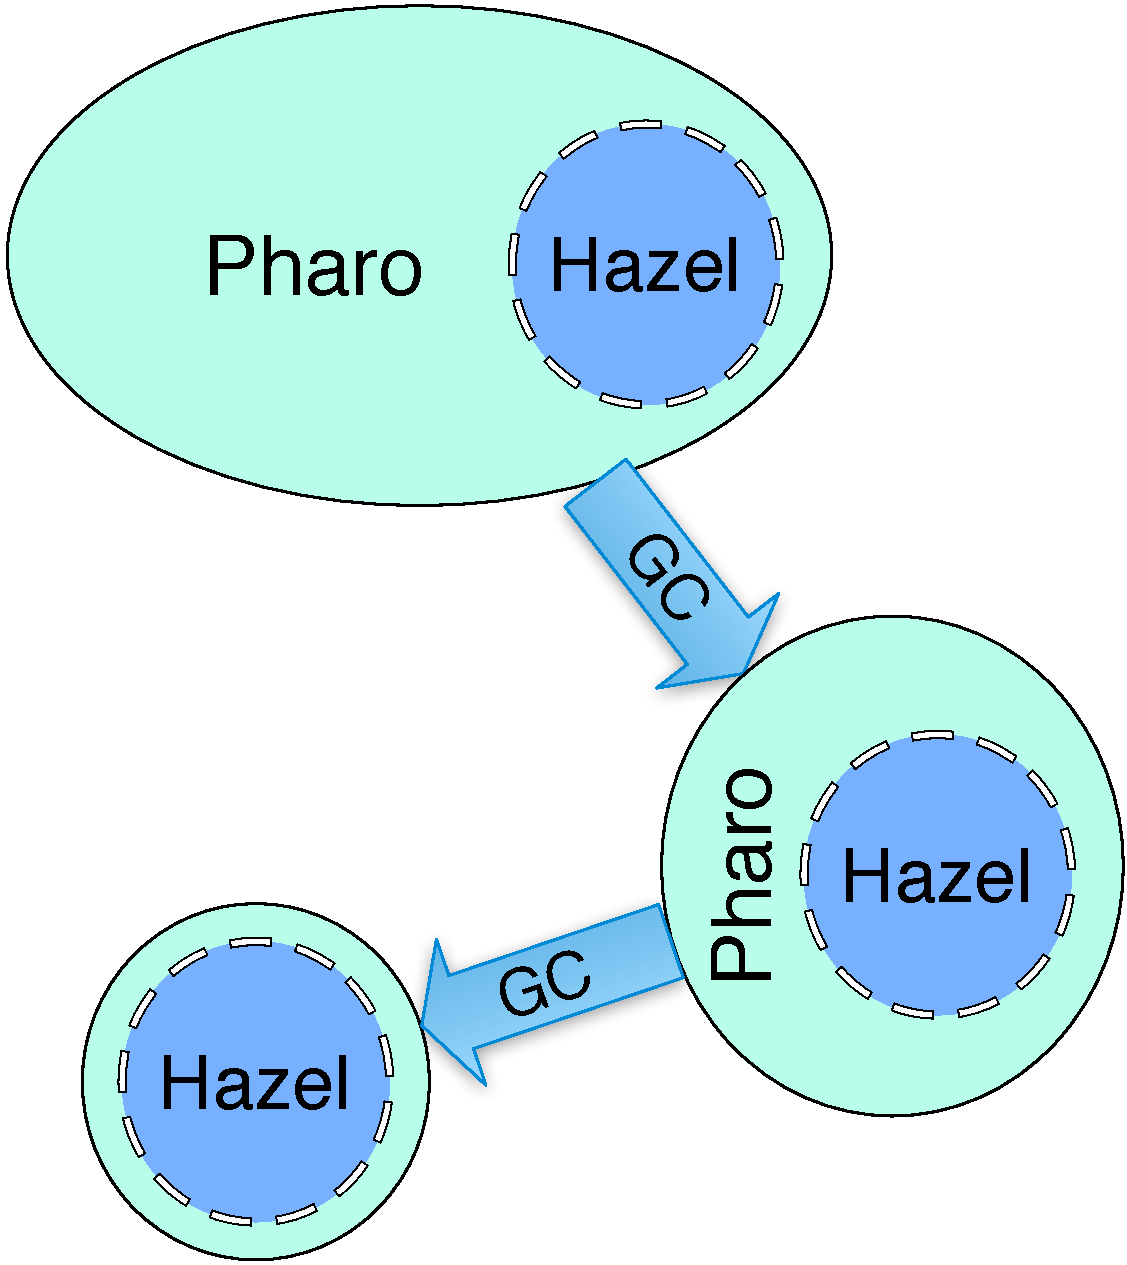
\includegraphics[width = 4.5cm]{figures/HazelSolution}
	\caption{Hazel - Garbage Collection of unneeded objects}
	\label{HazelSolution}
\end{figure}

Two solutions have been tested to create the image:
\begin{itemize}
	\item The first solution was to take a lively image and to dynamically switch the \gls{Special Objects Array} in order to make the unneeded object garbage collected (see \emph{\gls{Garbage Collector}} page~\pageref{glossary}). The difficulty of this method is that we are drastically modifying the image during its own execution. Some objects can easily be changed (i.e. \ct{nil} or \ct{Character}) when some others freeze the Virtual Machine (i.e. \ct{String} or \ct{Semaphore}). We think it's due to the fact that during the execution of the switching method, we are modifying the method context, and the Virtual Machine points to unaccessible pointers and we got an error\footnote{\ct{segmentation fault}} (see Figure~\ref{HazelSolution}).
	\begin{itemize}
		\item To replace the \gls{Special Objects Array}, the idea was to take the current \gls{Special Objects Array}, which is a \ct{Dictionary}, and to replace its values. The problem is that some values called all the time by the image are buffered in the Virtual Machine (those values are \ct{nil},\ct{true} and \ct{false}) and updated at the opening of the image. So we have decided to use the \glspl{primitive} \ct{become:} and \ct{becomeForward:} which basically switch references between the receiver and the argument.
		\item Because some objects can't easily be switched, we have considered another approach.
	\end{itemize}
	\item The second solution, which is also the \gls{Micro Squeak} solution, consists in collecting then serializing all the needed objects into a new image (see Figure~\ref{MSSolution}). But since the tool used for \gls{Micro Squeak} was not maintained anymore and based on a really old version of Pharo, first we had to make it works.
\end{itemize}

\inanutshell We can produce a new image based on the previously created kernel.